\subsection{Theoretical model of the inner knot (SK,YY)}

The discovery of the jet-torus structure of the inner Crab nebula coincided with the emergence of computer codes for relativistic MHD capable of dealing with highly relativistic magnetised flows \citep{ssk-godun99}.  This was most handy, as theoretical MHD models of the Crab Nebula allowed for reasonable ideas on the origin of the structure but could not address the problem rigorously due to the complicated nature of non-spherically symmetric flows.   The  key properties of pulsar winds giving rise to the jet-torus 
appearance of the nebula in these models  are 1) their anisotropy, with the wind power increasing towards the equatorial plane of the pulsar rotation 2) their magnetisation, with purely azimuthal magnetic aligned with the pulsar’s rotational axis.  The first property naturally leads to the torus component, whereas the second opens the possibility of magnetic collimation of the flow toward the polar axis. In fact, this collimation  mechanism fails for the wind itself, with possible exception for a tiny polar section, due to its highly super-magnetosonic motion. However, downstream of the wind termination shock the corresponding Mach number drops, the causal connectivity across the flow is restored and the magnetic hoop stress regains its collimating  potential.  Thus, in the MHD model the Crab’s jet is not present in the un-shocked pulsar wind but forms in the shocked part of the wind and thus already inside the nebula.    

The first computer-generated models of the Crab Nebula focused on the case of weakly magnetised pulsar wind, thus adopting the conclusions of the Rees-Gunn-Kennel-Coroniti theory \citep{rees-gunn-74,kc84a,kc84b}.  To the delight of theorists, the simulations confirmed the possibility of the separation of the post-shock flow into the equatorial (torus)  and polar (jets) components, provided the wind magnetisation parameter $\sigma$ exceeded the critical value of few$ \times 10^{-3}$ \citep{ssk-lyub-03,ssk-lyub-04,delzanna-04,bogovalov-05}.  This could be concluded immediately from the analysis of the velocity field and the distribution of other fluid parameters but in order to compared the results with the observations a synthetic emission map is highly desirable. Some elements required for the synchrotron emission calculations were readily provided by the numerical models. These are the magnetic field field strength and the orientation, as well as the velocity field, which is important for the relativistic beaming and Doppler effects.   The missing part, concerning the spectrum of the ultra-relativistic electrons, had to be recovered indirectly, via a crude model connecting the spectrum to the fluid pressure of the MHD solution\footnote{A more sophisticated technique was used in more recent simulations. }  The un-shocked wind zone was not expected to make a significant contribution and hence was explicitly excluded from the emission calculations.

One of the most prominent and yet unexpected features of the synthetic synchrotron images of the simulated PWN was 
a very bright feature located right in the centre, where the image of the model’s pulsar would be if its emission was included (but it was not, \cite{ssk-lyub-03,ssk-lyub-04}).  A closer look revealed that the feature was a slightly off-centred and extended knot.  In order to identify the feature of the synthetic images with a particular feature of the numerical solution,  a detailed inspection of the data was carried out and it revealed that the emission originated close to the termination shock, where the shocked wind plasma was still flowing with  (moderatly) relativistic speed towards the fiducial observer,  and for this reason was subject to significant 
Doppler-boosting.  This is illustrated in Figure~\ref{knot-mhd-model}. Subsequent  studies by other groups \cite{delzanna-06} and  the recent 3D simulations \citep{porth-13,porth-14} confirmed the result.       

%\begin{figure}[h!]
%\begin{center}
%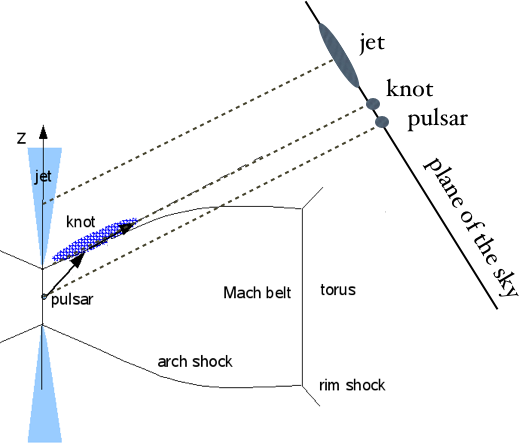
\includegraphics[width=0.7\columnwidth]{f2.png}
%\caption{In this sketch, we show the plane defined by the rotational axis of %the pulsar and the location of fiducial  observer.  The region around the %pulsar corresponds to the un-shocked  pulsar wind, the continuous lines show %the wind termination shock, indicating its topological components, the Mach %belt, arch and rim shocks. The blue shaded region shows the region there the %shocked wind plasma flows towards the observer with moderately relativistic %speed. The dashed lines are the lines of sight, which show the order in %which the jet the knot and the pulsar appear in the plane of the sky of the %observer.   
%}
%\end{center}
%\label{knot-mhd-model}
%\end{figure}

Once we had understood the nature of the feature, it became clear that a counterpart must be present in the real images of the Crab Nebula, unless something is very wrong with the MHD model. The oblate geometry of the termination shock ensures that there always be a shock section where the post-shock plasma is streaming towards the observer with relativistic speed and hence its emission is Doppler-boosted.   Provided the Crab’s synchrotron electrons are indeed accelerated at the termination shock, as proposed in the Kennel-Coroniti model, this ensures the existence of a bright knot inside the area occupied in the plane of the sky by the un-shocked pulsar wind zone.  This knot must be a very bright permanent feature, located on the projected symmetry axis. Since the polar jets are also subject of relativistic beaming, the knot must be on the jet side of the pulsar (see Figure~\ref{knot-mhd-model}) and have no counterpart on the counter-jet side.      
A comparison with the high-resolution HST images revealed that such a feature is indeed present  in the Crab Nebula: 
it is called the inner knot (or knot 1; \citet{hester-95}) and is located approximately 0.65 arcsec away from the Crab pulsar.  
So far it has been detected only in the optical-IR range.  The emission is strongly polarised with the electric polarisation vector aligned with the rotational axis in the plane of the sky. This is exactly what is expected as in the close vicinity of the termination shock the magnetic field should still preserve the highly regular azimuthal structure it has in the wind.  In a way, the inner knot was predicted by the simulations and then confirmed by the observations. Indeed, even if the observational discovery of the Crabs knot  preceded  the simulations, it was not immediately connected to the termination shock and its emergence in the synthetic maps was a complete surprise.       

The identification of the inner knot with the termination shock is already very interesting as it implies a unique opportunity for studying properties of highly relativistic shocks in magnetised plasma.  The discovery of gamma ray flares in the Crab Nebula added interest as the short life-time of the electrons emitting at such energies suggests that the gamma-ray emission originates from the terminations shock, provided it is the main acceleration site for the synchrotron electrons of all energies. Moreover, the beamed nature of the emission in this region ensures the domination of  the inner knot contribution to the observed 
gamma-ray flux \citep{ssk-lyut-11}.  Unfortunately, the angular resolution of gamma-ray telescopes is not sufficient to test this conclusion directly.  Under such circumstances, the only way to localise the flares is via their identification with structural variability in the radio, optical-IR and X-ray windows where the resolution of modern instruments is much higher. Such observations have been carried out but they have not led to a positive identification so far. Moreover, they seem to have ruled out the inner knot as the source of gamma-ray flares as its variability did not show any correlation with the flares \citep{Rudy-15}. On the other hand, these studies significantly  increased the available information on the knot properties, allowing to test its theoretical connection with termination shock in greater detail.      
    
The knot does not seem to have much of an internal structure, with brightness gradually decreasing from the peak value in the centre to the background one at the periphery. It is elongated in the direction normal to the rotational axis and a little bit bowed away from the pulsar. The knot is clearly separated from the pulsar and the separation varies with  a $30\%$ amplitude on the time scale of few months, which is similar to the wisp production time scale.   The knot’s flux anti-correlates with the separation.      
The variability implies that the in the vicinity of the termination shock the flow of shocked plasma is not steady but varies on the time-scale of the shock light-crossing time.  In fact, such a variability, accompanied by a strong variation of the shock geometry, was  discovered in numerical simulations before the observations. In the high-resolution 2D simulations by \citep{camus-09}, it was found that this variability led naturally to emergence of wisps in synthetic synchrotron maps.  These wisps were identified with inhomogeneities created by the variable shock in the  equatorial outflow and advected with the outflow speed.  Thus, the similar time scales of the inner knot dynamics and the wisp production are easily explained by the fact that both are traced back to the termination shock variability.  Moreover, the recent 3D simulations of the Crab nebula are consistent with the observed knot’s ``flux-separation’’ anti-correlation \citep{porth-14}.             

A couple of attempts have been made recently to build simple semi-analytical models of the Crab’s inner knot \citep{YB-15,LKP-16}. The main motivation behind these attempts is based on the fact that the structure of the upstream wind is relatively simple and one of the key factors determining the knot appearance, namely the Doppler beaming, is relatively easy to predict based on the properties of relativistic transverse MHD shock.  The most important conclusion of the studies is that the observed clear separation of the knot from the pulsar can only be achieved in models with low wind magnetisation ($\sigma \ll 1$).   
Indeed, suppose that the brightness peak of the knot corresponds to the point on the shock where the shocked plasma 
flows directly towards the observer. Then the observed angular distance between the peak and the pulsar is determined 
by flow deflection angle $\Delta\delta$ at the shock (see Figure~\ref{knot-separation}). The knot will not engulf the pulsar provided the half-opening angle of the Doppler beam, $\alpha_d$ is smaller than the deflection angle along the line of sight passing through the pulsar (see Figure~\ref{knot-separation}). Given the ultra-relativistic nature of the wind, both these angles depend mostly of the upstream $\sigma$ and hence the condition $\alpha_d < \Delta\delta$ translates into the condition on $\sigma$.    

The deduced low $\sigma$ is in contrast with the theoretical expectation of high $\sigma$ in pulsar winds. This conflict can be settled if the knot is produced by the striped equatorial section of the wind. In the striped section, $\sigma$ can be reduced via
magnetic dissipation of the stripes either in the wind or inside the hybrid MHD shock which terminates it, with the post-shock flow dynamics being identical for the alternatives.  


\begin{figure}[h!]
\begin{center}
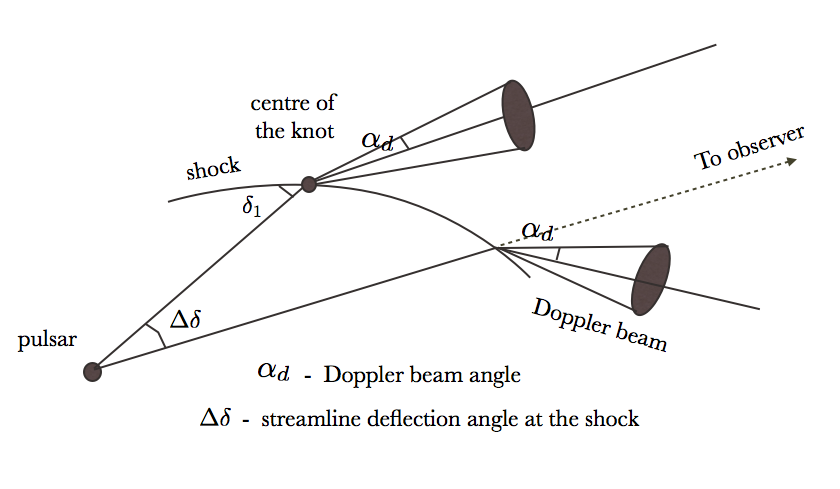
\includegraphics[width=0.7\columnwidth]{figures/f1/f1_original}
\caption{In this sketch, we show Doppler beams at two locations on the termination shock, selected by the lines of sight originated at the pulsar and  at the brightness peak of the knot, where the post-shock velocity is parallel to the line of sight.  
In order for the knot not to extend all the to the pulsar in the plane of the sky,  the Doppler beam at the first location should point away from the observer and hence $\alpha_d < \Delta\delta$.  
}
\end{center}
\label{knot-separation}
\end{figure}

Using the Doppler-beamed post-shock emissivity as a proxy for the knot brightness, one can estimate a number of observed  knot parameters such as the degree elongation, the distance from the pulsar in the units of the equatorial radius of the termination shock, and its polarisation degree.     The results are somewhat dependent on the  utilised model for the termination shock shape, but overall agree with the observational measurements quite well in the low-sigma-wind regime .  
The total flux polarisation degree is strongly effected by the relativistic aberration of light, which leads to a noticable rotation of the polarisation vector across the knot (see Figure~\ref{knot-polarisation}).  \citet{YB-15} concluded that the rotation imposes an upper limit 
of $\simeq 50\%$ on the overall polarisation degree of the knot, which is significantly lower than the observed $\simeq 60\%$ \sitep{moran-13}.  However, in the observations the integration was carried out only over a central part of the knot, thus excluding outer regions where the rotation is strong. \citep{LKP-16} have demonstrated that the polarisation decree decreases with the size of the integration area and this can explain the disagreement  between the observations and the upper limit found  in \citep{YB-15}.      
Moreover, the polarisation degree of the synthetic knot reproduced in the 3D simulation \citep{} agrees with the observed values exceptionally well. 

\begin{figure}[h!]
\begin{center}
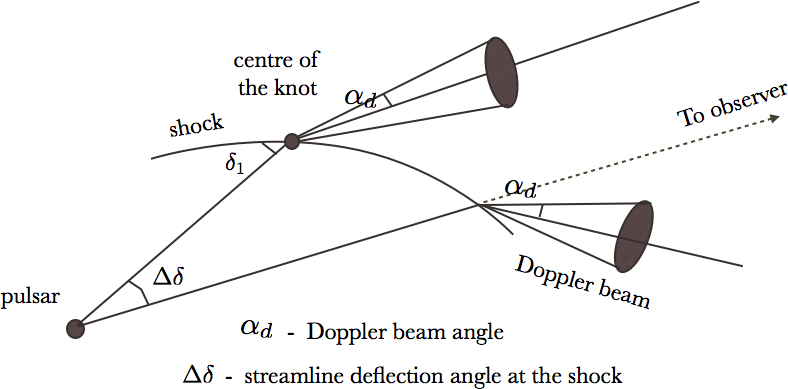
\includegraphics[width=0.7\columnwidth]{f3.png}
\caption{The emissivity distribution over the shock surface projected onto the plane of the sky and the polarisation vector of the shock emission. 
}
\end{center}
\label{knot-polarisation}
\end{figure}

The shape of the knot based on the emissivity isophotes was another matter of concern \citep{YB-15}. Instead being bowed away from the pulsar the knot looked bowed towards it, reflecting the shape of the termination shock ``shadow’’ in the plane of the sky (see Figure~\ref{knot-polarisation}). In order to understand the significance of this result one has to study the role of other factors influencing the the knot appearance. For example,  the effective geometric thickness of the emitting layer may have a strong impact as well as the variations of the velocity field in this layer \citep{LKP-16,YB-15}.  Figure~\ref{thickness-effect} illustrates the role of finite thickness for in a model where the emissivity above the termination shock is set via an extrapolation of that at the shock surface\citep{LKP-16}. One can see that the effect is rather strong.    

\begin{figure}[h!]
\begin{center}
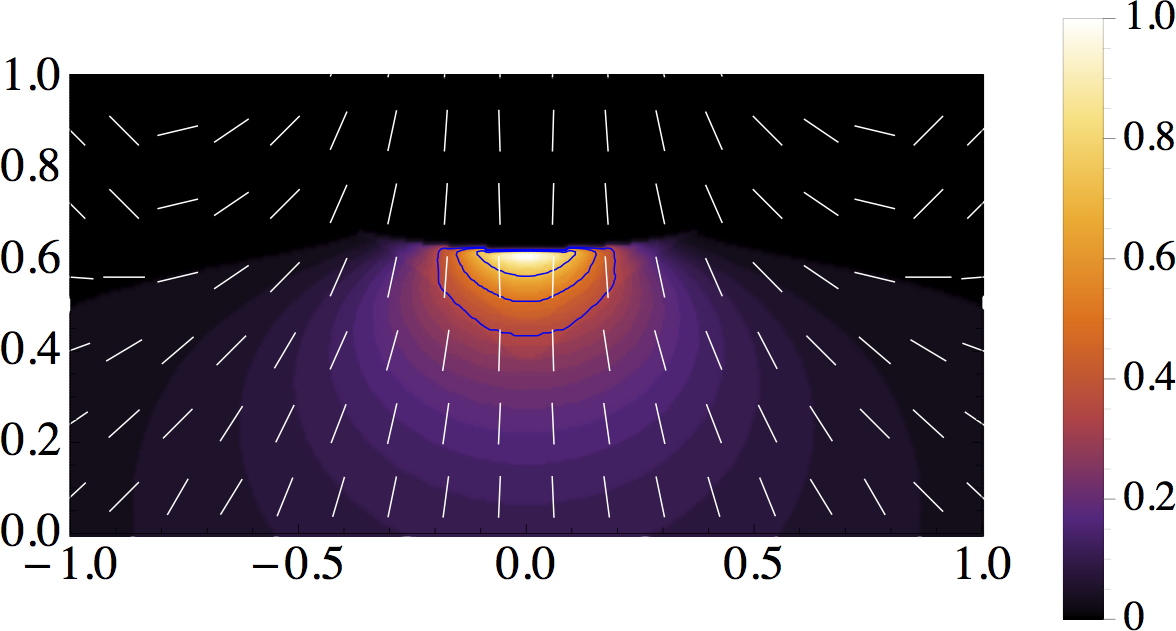
\includegraphics[width=0.99\columnwidth]{f4.png}
\caption{The top panels show the knot images resulting from emitting region of thickness equal to 0.1 (left) and 0.2 (right) of the local shock radius. The bottom panels illustrate the emissivity models used for these calculations. The dotted line shows the termination shock surface, the dashed line shows the line of sight and the mono-coloured image shows the corresponding volume emissivity distribution. 
}
\end{center}
\label{thickness-effect}
\end{figure}

In these calculations, it was assumed that the spectrum of the knot emission is a power law. This implies that the termination shock is an efficient accelerator of non-thermal particles. Although this assumption is a corner stone of the popular and successful model for the Crab Nebula emission by Kennel-Coroniti, its validity have been questioned by the PIC simulations of shocks in striped flow \citep{SS-11}. They suggest that the non-thermal particles acceleration can only be efficient in small equatorial sector where the downstream plasma becomes almost unmagnetised.  Otherwise, the plasma is simply heated and its synchrotron emission must have thermal spectrum.  Interestingly, the current failure to detect both the radio and X-ray emission from the knot  is consistent with such a spectrum.      

